\chapter{Introduction}
% Argumentation in general and in research.
We all encounter arguments in our lives frequently. When talking to friends, listening to political discussions, or even making decisions in our head. These arguments can get heated and complex since humans have different beliefs and motivations. Finding a common ground or a "correct" conclusion is complicated and sometimes impossible. However, these imperfections are what make us humans. \ac{AI}, conversely, needs to act precisely and logically \cite{DBLP:journals/frai/DietzKM24}. That is why much research is being done on knowledge representation and reasoning \cite{DBLP:journals/dagstuhl-manifestos/DelgrandeG0TW24, DBLP:journals/inffus/PopescuD23}.

% Abstraction of Argumentation -> promises and conclusions, attacks
When observing arguments objectively, we can distinguish between facts and conclusions. A fact represents a specific state in the real world. A conclusion on the other hand is a fact claimed by the logical relation of the promises. The relations are opposing facts (f.e. \emph{the square $x$ is red} and \emph{the square $x$ is blue}), which are contradicting each other. While accepting the correctness of facts is very important, refuting facts is even more critical in an argument.

% Abstract Models of argumentation. Graphs.
If a fact or, i.e., an argument $a$ is a counterargument of another argument $b$, we can say that $a$ attacks $b$. With this generalization, we can abstract our model with directed graphs. The arguments are represented as nodes, and the attacks as directed edges \cite{DUNG1995321}. With this abstraction, we can define \acp{AF} and use them to evaluate conclusions \cite{DBLP:conf/fapr/Geffner96}. Most of the time, we do not operate on real-world cases, but on abstract examples. This means, that we do not care about the argument which is represented by a specific node. But drawing a conclusion from an \ac{AF} can be challenging and tears down to the definition of semantics.

% Semantics with AFs
% Computation, complexity classes of computing sets
A semantic defines a subset of argument sets that satisfy the semantic-specific rules. Dung already defined different semantics \cite{Dung1995-DUNOTA-2} like \ac{cf}, \ac{adm} and \ac{stb}. According to Dungs definitions, a set \textit{S} is \ac{cf} if there are no attacks between the arguments in \textit{S}. The conflict-free set is mainly a building block for the other semantics, which means that the conflict-free set is always a superset of admissible and stable. 
A stable set, is a conflict-free set, if for every argument, which is not in \textit{S}, has an attacker which is in \textit{S}. 
Finally, an admissible set is a conflict-free set, where each argument in \textit{S} has a defender in \textit{S}. 
The specific rules can be defined via a boolean formula. They can be used to encode the \acp{AF} to be solvable with different boolean solvers like \ac{ASP} \cite{DBLP:journals/corr/abs-1301-1388} or, as in our case, with a \ac{SAT-Solver} \cite{DBLP:journals/amai/AmgoudD13}. Unfortunately, drawing a conclusion from an AF can be challenging, e.g., it can be NP-complete and sometimes even be beyond NP to decide whether an argument is acceptable under a specific argumentation semantics \cite{DBLP:journals/ai/DvorakGRW23}. In fact, the complexity of proofing faithfulness or spuriousness of an \ac{AF} is $\prod_2^P$ \cite{DBLP:conf/kr/SaribaturW21}. This means, that to obtain a result, multiple instances or calls of a SAT-Solver need to be invoked. 


% Clustering of AFs
One of the first papers describing the concept was written by Dung \cite{Dung1995-DUNOTA-2} in 1995. Since then, there has been more and more interest in \acp{AF} due to the artificial intelligence community \cite{DBLP:books/ox/22/CocarascuC0T22}. The argumentation systems and semantics have been modified and improved over the years, and another abstraction layer has been added. This specific abstraction layer is called \emph{clustering} and generalizes multiple arguments into one bundled cluster \cite{DBLP:conf/kr/SaribaturW21}. Clustering is a technique to reduce the number of arguments without changing the conclusion, which in this instance would be the sets produced by a specific semantic. When producing a clustered (\emph{abstract}) \ac{AF}, which produces the same semantic sets as the non-clustered (\emph{concrete}) \ac{AF}, the abstract \ac{AF} is defined to be \emph{faithful}. While each concrete semantic set has a directly mapped abstract semantic set, not every abstract semantic set has to have a directly mapped concrete semantic set. If we create an abstract \ac{AF} that produces a semantic set that cannot be mapped to a concrete semantic set, we call it \emph{spurious}.



% Importance of creating faithful abstract AFs
When reducing the amount of arguments with clustering we have to pay attention to not abstract crucial facts, and thus, falsify accepted sets from the concrete \ac{AF} or accept refuted ones. This would lead to a spurious abstraction and the abstract \ac{AF} would not represent the concrete \ac{AF} anymore. To preserve the representation of the concrete \ac{AF}, we need to show faithfulness.


% Example
For instance, let us consider a real-world example like the weather. We can define arguments:

\begin{itemize}
    \item $a$: The sky is blue
    \item $b$: The atmosphere scatters the sunlights and makes the sky appear blue. 
    \item $c$: There exist photographs of a blue sky. 
    \item $d$: Photographs can be fake.
    \item $e$: At sunrise the sky appears to be orange. 
    \item $f$: Observations can alter, depending on the time.
\end{itemize}

With this knowledge basis, we can create a concrete \ac{AF} $G = (A, R)$. Where we abstract the arguments into nodes and transform the opposing statement into attacks as shown in \ref{af:introExample1}. If we apply another layer of abstraction, we obtain, f.e. the abstract \ac{AF} $G' = (A', R')$ defined in \ref{af:introExample2}. Here we created a single Cluster consisting of the singletons \texttt{\{a, b, c, e, f\}}.



\vspace{0.3cm}
\begin{figure}[h]
\begin{minipage}{.5\textwidth}
    \centering
    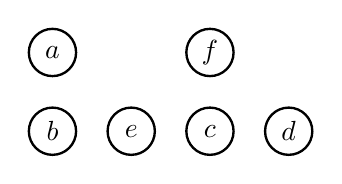
\begin{tikzpicture}
        % Singletons
        \def \ax{0}     \def \ay{0}
        \def \bx{0}     \def \by{-1}
        \def \cx{2}     \def \cy{-1}
        \def \dx{3}     \def \dy{-1}
        \def \ex{1}     \def \ey{-1}
        \def \fx{2}     \def \fy{0}

        \draw[line width=0.3mm] (\ax, \ay) circle (0.3) node[anchor=center]{$a$};
        \draw[line width=0.3mm] (\bx, \by) circle (0.3) node[anchor=center]{$b$};
        \draw[line width=0.3mm] (\cx, \cy) circle (0.3) node[anchor=center]{$c$};
        \draw[line width=0.3mm] (\dx, \dy) circle (0.3) node[anchor=center]{$d$};
        \draw[line width=0.3mm] (\ex, \ey) circle (0.3) node[anchor=center]{$e$};
        \draw[line width=0.3mm] (\fx, \fy) circle (0.3) node[anchor=center]{$f$};

        % Attacks
        \DrawAttackHorizontal{L}{\fx}{\fy}{\ax}{\ay}
        \DrawAttackHorizontal{B}{\ex}{\ey}{\bx}{\by}
        \DrawAttackHorizontal{B}{\cx}{\cy}{\ex}{\ey}
        \DrawAttackHorizontal{L}{\dx}{\dy}{\cx}{\cy}
        \DrawAttackVertical{D}{\fx}{\fy}{\cx}{\cy}
        \DrawAttackDiagonal{PB}{\fx}{\fy}{\ex}{\ey}
        \DrawAttackDiagonal{NB}{\ax}{\ay}{\ex}{\ey}
    \end{tikzpicture}
    \caption{\ac{AF} G concrete}
    \label{af:introExample1}
\end{minipage}%
\begin{minipage}{.5\textwidth}
    \centering
    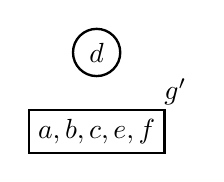
\begin{tikzpicture}
        % Singletons
        \def \gx{0}     \def \gy{-1}
        \def \dx{0}     \def \dy{0}

        \node[rectangle, draw, line width=0.3mm] at (\gx, \gy) {$a,b,c,e,f$};
        \node at (1, -0.5) {$g'$};
        \draw[line width=0.3mm] (\dx, \dy) circle (0.3) node[anchor=center]{$d$};

        % Attacks
        \DrawSelfAttackLeftTopCluster{\gx-0.8}{\gy + 0.3}
        \DrawAttackVertical{D}{\dx}{\dy}{\gx}{\gy}
    \end{tikzpicture}
    \caption{\ac{AF} G' abstract}
    \label{af:introExample2}
\end{minipage}
\end{figure}




Now we can compute the sets of the according semantic (\ac{cf}, \ac{adm}, \ac{stb}). To reduce cluttering, we keep this example to the stable semantic. The stable sets of the \ac{AF} $G$ defined in \ref{af:introExample1} are \texttt{stb=[\{d, e\}, \{b, d, f\}]}.

By computing the stable semantic sets of the abstract \ac{AF} $G'$ \texttt{stb=[\{d\}, \{d, g'\}]}, we can observe that it is spurious due to the extension \texttt{\{d\}}, since it cannot be mapped to one of the concrete stable extensions. 

When concretizing the argument \texttt{\{c\}}, we create a new \ac{AF} $G'' = (A'', R'')$ \ref{af:introExample3}, which has the following stable extensions: \texttt{stb=[\{g', d\}]}. This Extension can be mapped to both stable extensions of the concrete \ac{AF} $G$, by expanding the cluster \texttt{g'} with \texttt{\{e\}} or \texttt{\{b, f\}}. Thus, we created a faithful abstract \ac{AF}.

\begin{figure}[h]
    \centering
    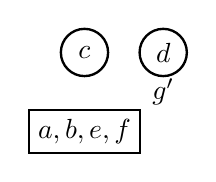
\begin{tikzpicture}
        % Singletons
        \def \gx{0}     \def \gy{-1}
        \def \dx{1}     \def \dy{0}
        \def \cx{0}     \def \cy{0}

        \node[rectangle, draw, line width=0.3mm] at (\gx, \gy) {$a,b,e,f$};
        \node at (1, -0.5) {$g'$};
        \draw[line width=0.3mm] (\dx, \dy) circle (0.3) node[anchor=center]{$d$};
        \draw[line width=0.3mm] (\cx, \cy) circle (0.3) node[anchor=center]{$c$};

        % Attacks
        \DrawSelfAttackLeftTopCluster{\gx-0.65}{\gy + 0.3}
        \DrawAttackHorizontal{L}{\dx}{\dy}{\cx}{\cy}
        \DrawAttackVertical{B}{\cx}{\cy}{\gx}{\gy}
    \end{tikzpicture}
    \caption{\ac{AF} G''}
    \label{af:introExample3}
\end{figure}


% Importance of concretizing single arguments
When producing an \ac{AF} with multiple layer of abstractions, the concrete problem can be hard to map. To still have an understanding of the structure to some extend, extracting single arguments of the cluster by concretizing them can be helpful. This also allows the user to have a direct impact to the outcome and produce customized faithful \acp{AF}.  


% What we want to show in this paper
% Main contributions in this paper
Creating abstract, faithful \acp{AF} can be challenging and is the main focus of this paper. We created one of the first tools \cite{Pasero2024-AFClustering-Repo} to produce an abstract \acp{AF} based on a concrete \acp{AF}. We cover different setups and usages, including different semantics and base functionalities:

\begin{itemize}
    \item Generate semantic sets of a concrete- or abstract \ac{AF}. The sets calculated iteratively or all at once. The covered semantics are \ac{cf}, \ac{adm}, and \ac{stb}, which can be selected throughout the project independently by a parameter in the command line.

    \item Determine faithfulness or spuriousness by providing two \acp{AF}. We provide two approaches, \ac{BFS} and \ac{DFS}, which alter the procedure. While \ac{BFS} calculates all the semantic sets of the two \acp{AF} first and then compares them, \ac{DFS} calculates iteratively a semantic set of the abstract \ac{AF} and then verifies it with the concrete \ac{AF}. The algorithm selection is done via a command line parameter.

    \item Concretize a set of arguments (i.e., pull out arguments from the cluster) given the concrete \ac{AF} and an abstract \ac{AF} (faithful or spurious), and provide faithfulness (by concretizing other arguments not specified in the concretize list as well). The user provides the concretized arguments via a command line parameter.

    \item $\cdots$
\end{itemize}

\noindent

\textit{TODO: Further contributions}

\textit{TODO: give pointers to why are non-trivial to obtain}

\textit{TODO: Choice of methods to obtain results}

\textit{TODO: How big AFs are still feasible to solve}
